\documentclass[journal]{vgtc}                % final (journal style)
%\documentclass[review,journal]{vgtc}         % review (journal style)
%\documentclass[widereview]{vgtc}             % wide-spaced review
%\documentclass[preprint,journal]{vgtc}       % preprint (journal style)

%% Uncomment one of the lines above depending on where your paper is
%% in the conference process. ``review'' and ``widereview'' are for review
%% submission, ``preprint'' is for pre-publication, and the final version
%% doesn't use a specific qualifier.

%% Please use one of the ``review'' options in combination with the
%% assigned online id (see below) ONLY if your paper uses a double blind
%% review process. Some conferences, like IEEE Vis and InfoVis, have NOT
%% in the past.

%% Please note that the use of figures other than the optional teaser is not permitted on the first page
%% of the journal version.  Figures should begin on the second page and be
%% in CMYK or Grey scale format, otherwise, colour shifting may occur
%% during the printing process.  Papers submitted with figures other than the optional teaser on the
%% first page will be refused. Also, the teaser figure should only have the
%% width of the abstract as the template enforces it.

%% These few lines make a distinction between latex and pdflatex calls and they
%% bring in essential packages for graphics and font handling.
%% Note that due to the \DeclareGraphicsExtensions{} call it is no longer necessary
%% to provide the the path and extension of a graphics file:
%% 
\includegraphics{diamondrule} is completely sufficient.
%%
\ifpdf%                                % if we use pdflatex
  \pdfoutput=1\relax                   % create PDFs from pdfLaTeX
  \pdfcompresslevel=9                  % PDF Compression
  \pdfoptionpdfminorversion=7          % create PDF 1.7
  \ExecuteOptions{pdftex}
  \usepackage{graphicx}                % allow us to embed graphics files
  \DeclareGraphicsExtensions{.pdf,.png,.jpg,.jpeg} % for pdflatex we expect .pdf, .png, or .jpg files
\else%                                 % else we use pure latex
  \ExecuteOptions{dvips}
  \usepackage{graphicx}                % allow us to embed graphics files
  \DeclareGraphicsExtensions{.eps}     % for pure latex we expect eps files
\fi%

%% it is recomended to use ``\autoref{sec:bla}'' instead of ``Fig.~\ref{sec:bla}''
\graphicspath{{figures/}{pictures/}{images/}{./}} % where to search for the images

\usepackage[UTF8]{CTEX}
\usepackage{microtype}                 % use micro-typography (slightly more compact, better to read)
\PassOptionsToPackage{warn}{textcomp}  % to address font issues with \textrightarrow
\usepackage{textcomp}                  % use better special symbols
\usepackage{mathptmx}                  % use matching math font
\usepackage{times}                     % we use Times as the main font
\renewcommand*\ttdefault{txtt}         % a nicer typewriter font
\usepackage{cite}                      % needed to automatically sort the references
\usepackage{tabu}                      % only used for the table example
\usepackage{booktabs}                  % only used for the table example
\usepackage{graphicx}
\usepackage{caption}
\usepackage{subcaption}
\usepackage{fontspec}%% load unicode fonts
\usepackage{pdfpages}
\usepackage[vlined,ruled,commentsnumbered,linesnumbered]{algorithm2e}
%% We encourage the use of mathptmx for consistent usage of times font
%% throughout the proceedings. However, if you encounter conflicts
%% with other math-related packages, you may want to disable it.
%% In preprint mode you may define your own headline.
%\preprinttext{To appear in IEEE Transactions on Visualization and Computer Graphics.}

%% If you are submitting a paper to a conference for review with a double
%% blind reviewing process, please replace the value ``0'' below with your
%% OnlineID. Otherwise, you may safely leave it at ``0''.
\onlineid{0}

%% declare the category of your paper, only shown in review mode
\vgtccategory{Research}
%% please declare the paper type of your paper to help reviewers, only shown in review mode
%% choices:
%% * algorithm/technique
%% * application/design study
%% * evaluation
%% * system
%% * theory/model
\vgtcpapertype{please specify}

%% Paper title.
\title{公司内部威胁情报分析}

%% This is how authors are specified in the journal style

%% indicate IEEE Member or Student Member in form indicated below
%\author{Roy G. Biv, Ed Grimley, \textit{Member, IEEE}, and Martha Stewart}
%\authorfooter{
%% insert punctuation at end of each item
%\item
% Roy G. Biv is with Starbucks Research. E-mail: roy.g.biv@aol.com.
%\item
% Ed Grimley is with Grimley Widgets, Inc.. E-mail: ed.grimley@aol.com.
%\item
% Martha Stewart is with Martha Stewart Enterprises at Microsoft
% Research. E-mail: martha.stewart@marthastewart.com.
%}

%other entries to be set up for journal
\shortauthortitle{Biv \MakeLowercase{\textit{et al.}}: Global Illumination for Fun and Profit}
%\shortauthortitle{Firstauthor \MakeLowercase{\textit{et al.}}: Paper Title}

%% Abstract section.
\abstract{
} % end of abstract

%% Keywords that describe your work. Will show as 'Index Terms' in journal
%% please capitalize first letter and insert punctuation after last keyword
\keywords{大数据, 安全, 可视化, 数据分析, 可视分析}

%% ACM Computing Classification System (CCS). 
%% See <http://www.acm.org/class/1998/> for details.
%% The ``\CCScat'' command takes four arguments.

%\CCScatlist{ % not used in journal version
% \CCScat{K.6.1}{Management of Computing and Information Systems}%
%{Project and People Management}{Life Cycle};
% \CCScat{K.7.m}{The Computing Profession}{Miscellaneous}{Ethics}
%}

%% Uncomment below to include a teaser figure.
\teaser{
  \centering
  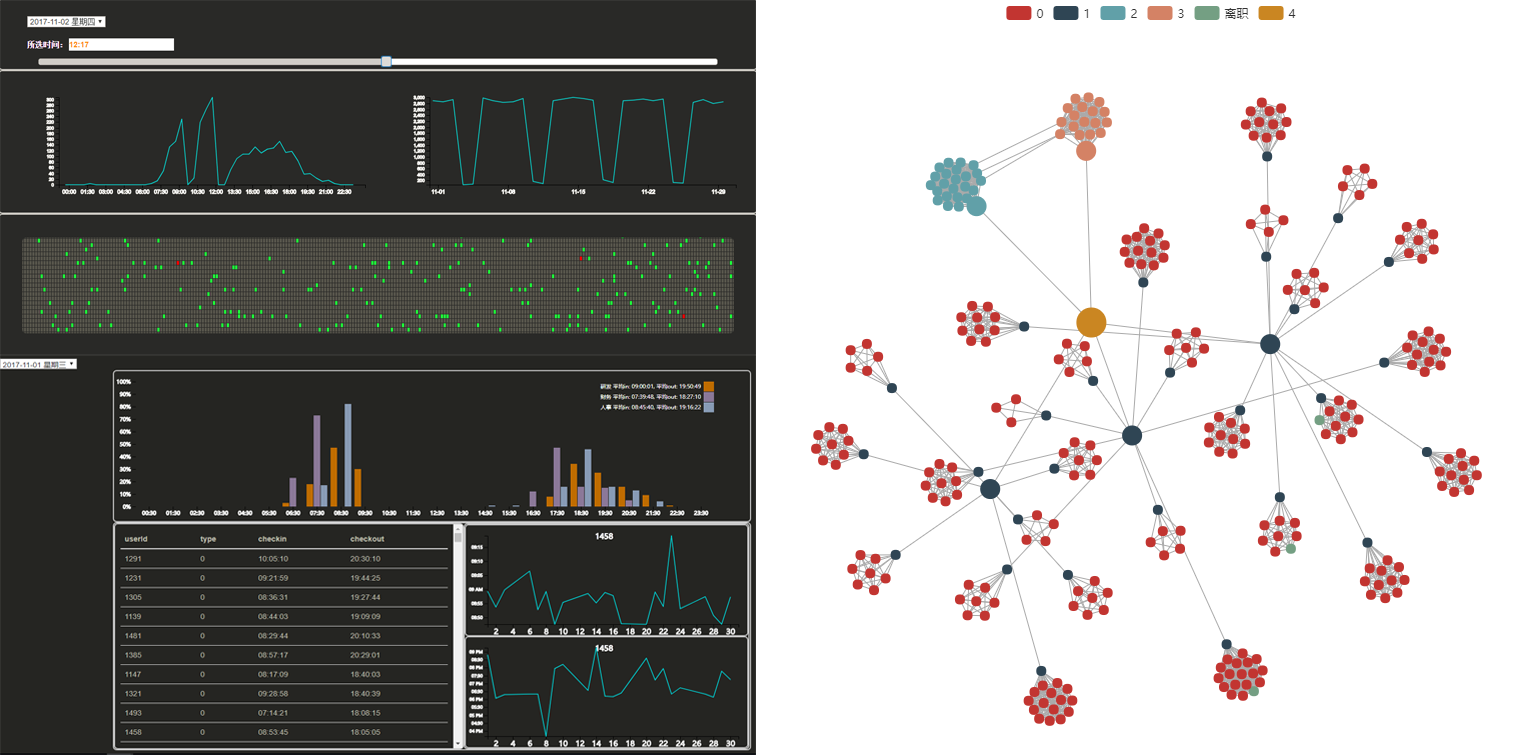
\includegraphics[width=\linewidth]{pictures/abstract.png}
  \caption{概要:按逆时针方向从左上图分别表示xx, 签到情况, 邮件往来情况}
	\label{fig:teaser}
}

%% Uncomment below to disable the manuscript note
%\renewcommand{\manuscriptnotetxt}{}

%% Copyright space is enabled by default as required by guidelines.
%% It is disabled by the 'review' option or via the following command:
% \nocopyrightspace

%\vgtcinsertpkg

%%%%%%%%%%%%%%%%%%%%%%%%%%%%%%%%%%%%%%%%%%%%%%%%%%%%%%%%%%%%%%%%
%%%%%%%%%%%%%%%%%%%%%% START OF THE PAPER %%%%%%%%%%%%%%%%%%%%%%
%%%%%%%%%%%%%%%%%%%%%%%%%%%%%%%%%%%%%%%%%%%%%%%%%%%%%%%%%%%%%%%%%

\begin{document}

%% The ``\maketitle'' command must be the first command after the
%% ``\begin{document}'' command. It prepares and prints the title block.

%% the only exception to this rule is the \firstsection command
\firstsection{介绍}

\maketitle

我们的论文展示了数据可视分析挑战赛的结果。我们的目的是分析一家互联网高科技公司HighTech,有几百名员工,分属财务、人力资源和研发三个部门。公司高层决定临时成立内部威胁情报分析小组,该小组将根据公司内部采集到的数据,分析并处置可能存在的各种安全威胁。在分析威胁情报过程中,数据的复杂性需要计算智能处理,但发现和处置安全威胁需要人的经验、认知和判断,可视分析技术能将计算智能与人类智慧紧密结合,是威胁情报人员高效分析和理解威胁情报数据的利器。假设您是威胁情报分析小组的成员,我们的项目设计并实现了一套可视分析解决方案,帮助该公司及时准确地找出可能存在的内部威胁情报。

\section{我们的方案}
\subsection{平行坐标图}
平行坐标图将数据表中的每一行映射为线或剖面。某行的各个属性由线上的点表示。平行坐标图中的值始保持正常化,最低值绘制为 $0\%$,最高值绘制为 $100\%$。这表示对于沿 X 轴的每个点来说,相应的列中的最低值沿 Y 轴被设置为 $0\%$,此列中的最高值被设置为 $100\%$。各列的刻度完全独立,因此不要将某一列中曲线的高度与其他列中曲线的高度进行比较。

平行坐标对多维数据的表达是数据可视化的重要方法之一。它实现了多维数据在二维平面上的表示。利用平行坐标对数据进行分析处理的技术已经取得了很大的进展, 如刷( Brushing) 技术、交换坐标轴、抽象等。这些分析技术已经应 用到数据挖掘的很多领域,尤其在聚类分析中,平行坐标对数据集的定性分析使聚类结果的合理性得到证明。

其思想就是将$N$维数据点映射到处于$N$条平行的坐标轴上的彼此相连的$N-1$条线段。这 $N - 1$条线段与 $N$ 条 轴相交的$N$个点分别代表了数据点的$N$维数据。这条代表 $N$ 维数据的折线可用 $N -1$个线性无关的方程所表示, 方程公式\ref{equ:1}:
\begin{equation}
\label{equ:1}
\frac{x_1-a_1}{u_1}=\frac{x_2-a_2}{u_2}=\cdots = \frac{x_n-a_n}{u_n}
\end{equation}
\begin{equation}
\label{equ:2}
x_{i+1} = m_ix_i+b_i, \quad i = 1, 2, \cdots, n-1
\end{equation}
其中,$m_i = u_{i+1} / u_i$ 表示斜率,$b_i = (a_{i+1} - m_ia_i)$表示在$x_ix_{i+1}$平面中$x_{i+1}$轴上的截距。
\subsection{弦图}
弦图(Chord Diagram),弦图 (Chord Diagram) 可以显示不同实体之间的相互关系和彼此共享的一些共通之处,因此这种图表非常适合用来比较数据集或不同数据组之间的相似性。节点围绕着圆周分布,点与点之间以弧线或贝塞尔曲线彼此连接以显示当中关系,然后再给每个连接分配数值(通过每个圆弧的大小比例表示)。此外,也可以用颜色将数据分成不同类别,有助于进行比较和区分。线的粗细表示权重。

我们用弦图表示了一个时间段内两个IP地址之间的流量。

\subsection{力导引图}
力引导布局最早由Peter Eades在1984年的“启发式画图算法”一文中提出,目的是减少布局中边的交叉,尽量保持边的长度一致。此方法借用弹簧模型模拟布局过程:用弹簧模拟两个点之间的关系,受到弹力的作用后,过近的点会被弹开而过远的点被拉近;通过不断的迭代,整个布局达到动态平衡,趋于稳定。其后,“力引导”的概念被提出,演化成力引导布局算法FR(Fruchterman-Reingold算法)——丰富两点之间的物理模型,加入点之间的静电力,通过计算系统的总能量并使得能量最小化,从而达到布局的目的。这种改进的能量模型,可看成弹簧模型的一般化。

对于图中,节点$i$和$j$,用$d(i,j)$表示两个点的欧式距离,$s(i,j)$表示弹簧的自然长度,$k$是弹力系数,$r$表示两个点之间的静电力常数,$w$是两个点之间的权重。

弹簧模型如公式\ref{equ:3}:
\begin{equation}
\label{equ:3}
E_s = \sum_{i=1}^{n}\sum_{j=1}^{n}\frac{1}{2}k(d(i,j)-s(i,j))^2
\end{equation}

能量模型如公式\ref{equ:4}
\begin{equation}
\label{equ:4}
E=E_s+\sum_{i=1}^{n}\sum_{j=1}^{n}\frac{rw_iw_j}{d(i,j)^2}
\end{equation}

力引导图的伪代码如算法\ref{alg:1}:

\begin{algorithm}
	\BlankLine
	\caption{力引导布局伪代码}\label{alg:1}
	\BlankLine
	设置节点的初始速度为$(0,0)$\\
	设置节点的初始位置为任意但不重叠的位置\\
	
	\For{总动能=0;对每一个节点i;进行循环}
	{
		静力 $f=(0,0)$\\
		\For{对每一个出该节点外的每个节点$j$}
		{
			静力$f$=静力$f$+$j$节点对应$i$节点的库仑斥力
		}
		\For{对该节点上的每个弹簧s}
		{
			静力$f$=静力$f$+弹簧对该节点的胡克弹力
		}
		该节点速度=(该节点速度+步长*净力)*阻尼\\
		该节点位置=该节点位置+步长*该节点速度\\
		总动能=总动能+该节点质量*(该节点速度)$^2$
	}

	
\end{algorithm}

\section{实验及结论}
\begin{figure}
	\centering
	\begin{subfigure}{\linewidth} % width of left subfigure
		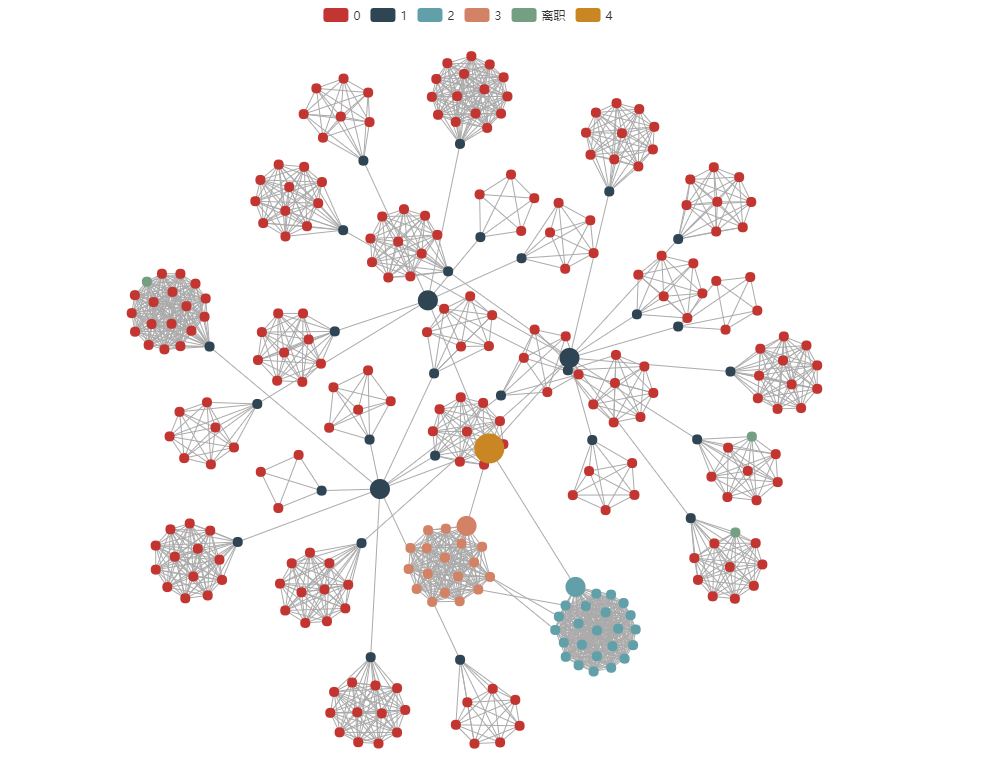
\includegraphics[width=\textwidth]{pictures/5-1.png}
		\caption{所有邮件数据的可视化} % subcaption
		\label{fig:all_category}
	\end{subfigure}
	%\vspace{1em} % here you can insert horizontal or vertical space
	\begin{subfigure}{0.3\linewidth} 
		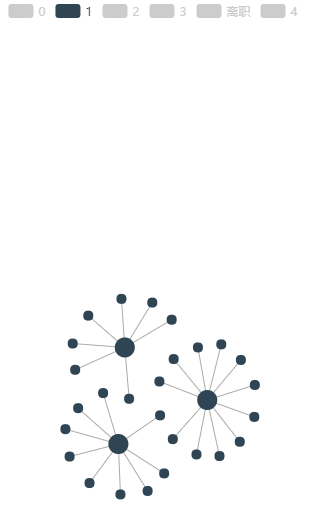
\includegraphics[width=\linewidth]{pictures/5-2.png}
		\caption{研发部中层管理} % subcaption
		\label{fig:med}
	\end{subfigure}
	\begin{subfigure}{0.3\linewidth} % width of right subfigure
		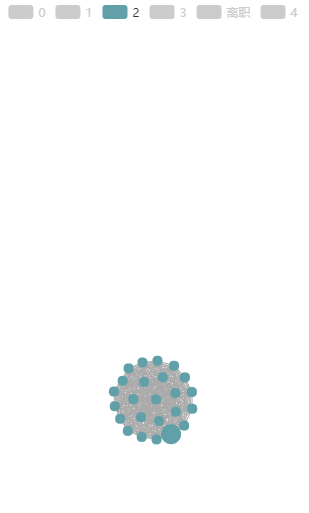
\includegraphics[width=\linewidth]{pictures/5-3.png}
		\caption{财务部所有职员} % subcaption
		\label{fig:finance}
	\end{subfigure}
	\begin{subfigure}{0.3\linewidth} % width of right subfigure
		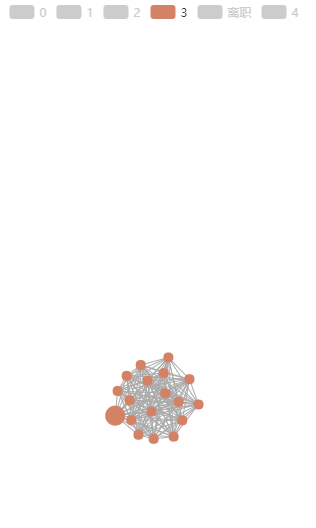
\includegraphics[width=\linewidth]{pictures/5-4.png}
		\caption{人力资源部所有职员} % subcaption
		\label{fig:hr}
	\end{subfigure}
	\caption{邮件数据分类别可视化结果} % caption for whole figure
\end{figure}

从邮件往来角度分析,整个的组织架构见图\ref{fig:all_category},中间黄色的是公司最高领导,只有一位,他直接管理中层领导。中间大小的蓝色圆是研发部部长,小一点的蓝色圆是小组长,红色的小圆是组员,绿色的小圆是离职的员工,之间的连线表示邮件往来。图\ref{fig:all_category}提供了所有数据的概览。

\subsection{财务部门}
财务部人员组成如图\ref{fig:finance}所示,可见财务部有一位主管,所有普通员工都向该主管汇报。

\subsection{人力资源部门}
人力资源部人员组成如图\ref{fig:hr}所示,可见人力资源部中也有一位主管。
从图\ref{fig:parrell}得知,人力资源部门对门户网站(如yahoo,sohu,huanqiu,hupu,163),购物网站(如taobao,amazon)的访问频率远高于其他部门。
\subsection{研发部门}
从图\ref{fig:parrell}, 公司代码相关的git服务器、jira(JAVA管理系统)和库服务器等,全是研发部在访问。
中层管理人员的情况如图\ref{fig:med}所示,可见中层管理人员分为两级,有小组长和研发部部长。观察所有组员的信息,可以发现,员工有组成小组的趋势。
\subsection{特点}
\begin{figure}
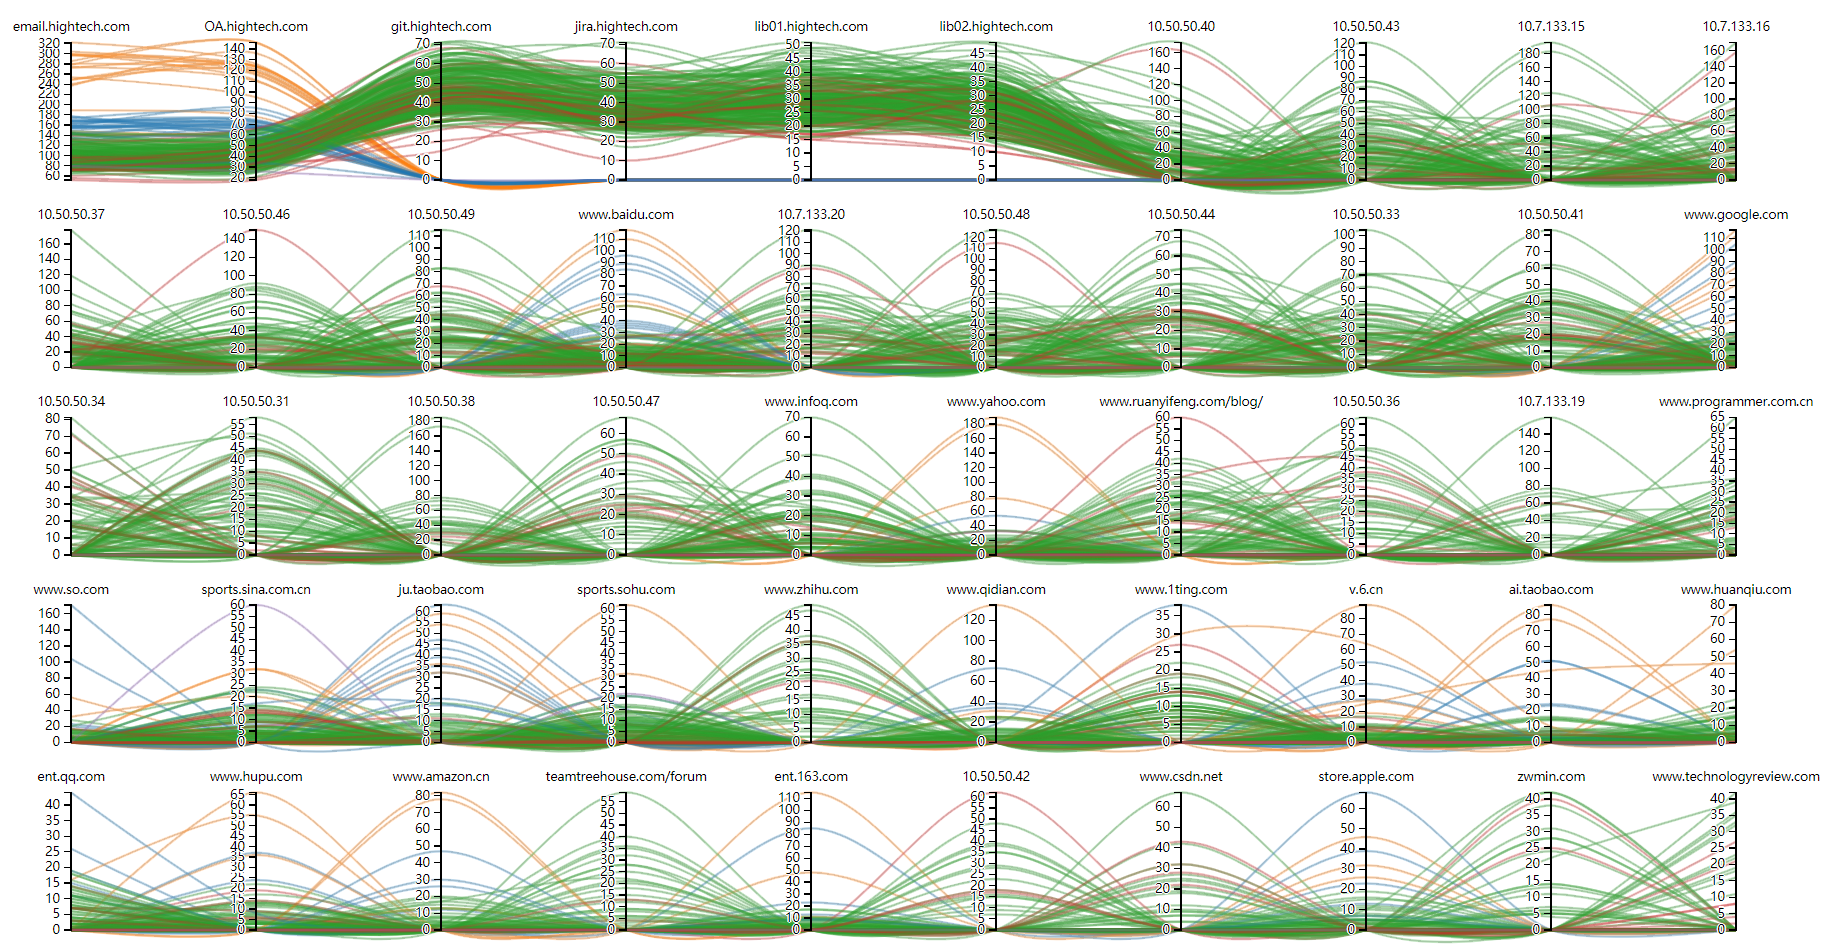
\includegraphics[width=\linewidth]{pictures/6.png}
\caption{平行坐标图分析}
\label{fig:parrell}
\end{figure}

%\bibliographystyle{abbrv}
%\bibliographystyle{abbrv-doi}
%\bibliographystyle{abbrv-doi-narrow}
%\bibliographystyle{abbrv-doi-hyperref}
%\bibliographystyle{abbrv-doi-hyperref-narrow}

%\bibliography{template}
\end{document}

